%\documentclass[aspectratio=43]{beamer}
%\documentclass[aspectratio=169]{beamer}
\documentclass[aspectratio=1610,12pt]{beamer}
\usepackage[utf8]{inputenc}
\usepackage[T1]{fontenc}
\usepackage{lmodern}

\usepackage[ngerman]{babel}
%\usepackage[ngerman]{babel} %use this for German presentations
\usepackage{booktabs} % fancy tables
\usepackage{tabulary} % tables with auto column length
\usepackage{hyperref}
\newcommand{\enquote}[1]{{\glqq#1\grqq{}}}

\usepackage{tikz}
\usepackage{xcolor}
\usetikzlibrary{decorations.text}
\definecolor{mygray}{RGB}{208,208,208}
\definecolor{myred}{HTML}{FF0000}
\definecolor{mypink}{HTML}{FF8080}
\definecolor{mygreen}{HTML}{80FF80}
\newcommand*{\mytextstyle}{\sffamily\normalfont\bfseries\color{black!85}}
\newcommand{\arcarrow}[4]{%
   % inner radius, middle radius, outer radius, start angle,
   % end angle, tip protusion angle, options, text
   \pgfmathsetmacro{\rin}{2.5}
   \pgfmathsetmacro{\rmid}{3.0}
   \pgfmathsetmacro{\rout}{3.5}
   \pgfmathsetmacro{\astart}{#1}
   \pgfmathsetmacro{\aend}{#2}
   \pgfmathsetmacro{\atip}{5}
   \fill[#4, very thick] (\astart+\atip:\rin)
                         arc (\astart+\atip:\aend:\rin)
      -- (\aend-\atip:\rmid)
      -- (\aend:\rout)   arc (\aend:\astart+\atip:\rout)
      -- (\astart:\rmid) -- cycle;
   \path[
      decoration = {
         text along path,
         text = {|\mytextstyle|#3},
         text align = {align = center},
         raise = -1.0ex
      },
      decorate
   ](\astart+\atip:\rmid) arc (\astart+\atip:\aend+\atip:\rmid);
}
\newcommand{\barcarrow}[4]{%
   % inner radius, middle radius, outer radius, start angle,
   % end angle, tip protusion angle, options, text
   \pgfmathsetmacro{\rin}{3.9}
   \pgfmathsetmacro{\rmid}{4.4}
   \pgfmathsetmacro{\rout}{4.9}
   \pgfmathsetmacro{\astart}{#1}
   \pgfmathsetmacro{\aend}{#2}
   \pgfmathsetmacro{\atip}{5}
   \fill[#4, very thick] (\astart+\atip:\rin)
                         arc (\astart+\atip:\aend:\rin)
      -- (\aend-\atip:\rmid)
      -- (\aend:\rout)   arc (\aend:\astart+\atip:\rout)
      -- (\astart:\rmid) -- cycle;
   \path[
      decoration = {
         text along path,
         text = {|\mytextstyle|#3},
         text align = {align = center},
         raise = -1.0ex
      },
      decorate
   ](\astart+\atip:\rmid) arc (\astart+\atip:\aend+\atip:\rmid);
}


# 6 arguments with 6 colors for 6 rings
# order: model, storage, query, browse, search, quality
\newcommand{\cycle}[6]{%
\begin{tikzpicture}
   \fill[even odd rule,myred] circle (1.5);

   \node at (0,0) [
      font  = \mytextstyle,
      color = white,
      align = center
   ]{
      HITO \\Lifecycle
   };
   \arcarrow{110}{50}{~~~Model}{#1}
   \arcarrow{40}{0}{~~~Storage}{#2}
   \arcarrow{-60}{-5}{Query~~}{#3}

   \arcarrow{-115}{-60}{Browse~~}{#4}
   \arcarrow{-120}{-200}{~~~Search/Explore}{#5}
   \arcarrow{-210}{-240}{~~~~Quality~}{#6}

   \barcarrow{110}{50}{~~~~~~Instance Generator~~}{#1}
   \barcarrow{40}{0}{~~~~GitHub}{#2}
   \barcarrow{-60}{-5}{Virtuoso~~}{#3}

   \barcarrow{-110}{-60}{LodView~~}{#4}
   \barcarrow{-115}{-190}{~~~~~Faceted Search, SNIK Graph~}{#5}
   \barcarrow{-200}{-240}{~~~~~HITO Quality}{#6}

\end{tikzpicture}
}

\usetheme{imise2}
\author{Franziska Jahn, Maryam Ghalandari, Konrad Höffner \& Thomas Pause}
\date{Leipzig, 15.Mai 2020}
\title{HITO}
\subtitle{MEDFLOSS Workshop}
\def\address{Härtelstraße 16-18, 04107 Leipzig}
\def\email{vorname.nachname@imise.uni-leipzig.de}
\def\telephone{~}

\usepackage{setspace}
\begin{document}
\begin{frame}
\titlepage
\end{frame}

\begin{frame}{Einleitung und Status von HITO}
  \centering
  \huge Franziska's Teil
\end{frame}

\begin{frame}{Agenda}
\begin{spacing}{1.25}
\begin{enumerate}
\item Einleitung und Status von HITO
\item Instance Generator: Eingabewerkzeug für MEDFLOSS Produkte in HITO
\item Kataloge und Zitate
\item Werkzeuge für die Navigation durch HITO
\item Szenarien für die Integration von medfloss.org und HITO
\item Diskussion
\end{enumerate}
\end{spacing}
\end{frame}

\begin{frame}{Das O in HITO -- Die Ontologie}
\centering
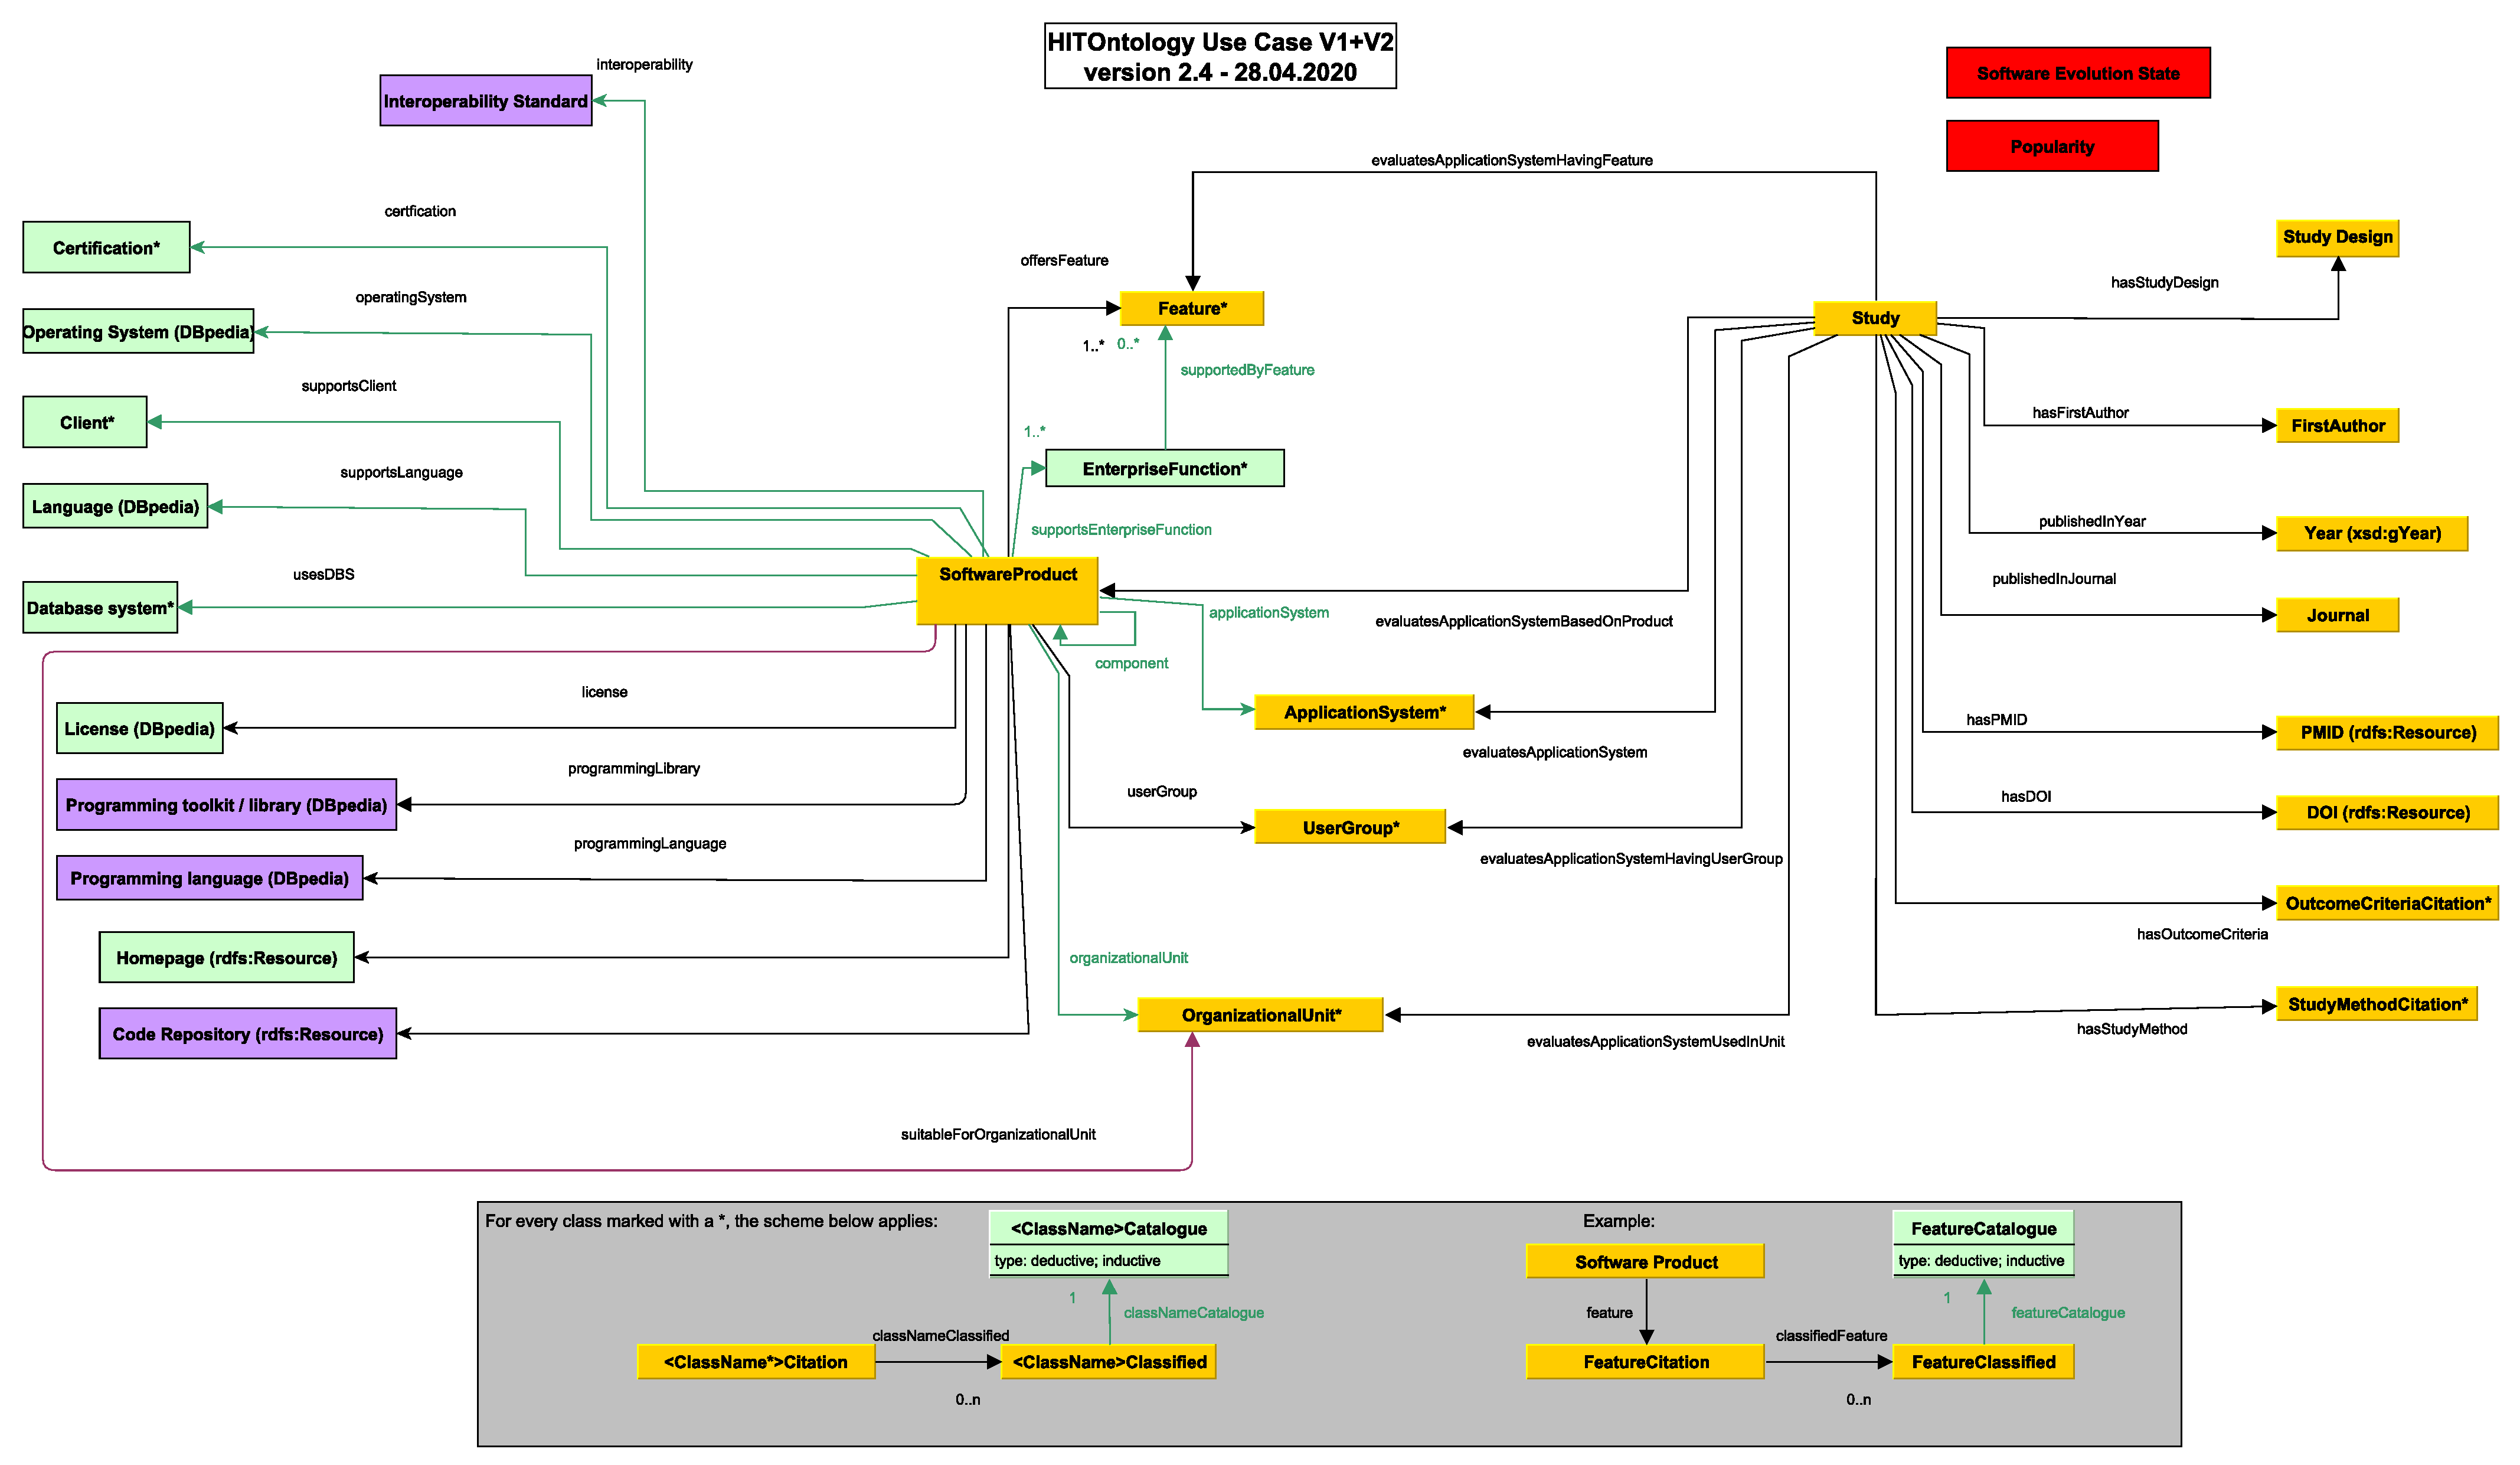
\includegraphics[width=.95\textwidth]{img/HITontology.pdf}
\end{frame}

\begin{frame}{Software Products in HITO}
\centering
\includegraphics[height=.8\textheight]{img/excerpt2.pdf}
\end{frame}

\begin{frame}{Fragen?}
  \centering
  \vspace{-0.5cm}
  \includegraphics[width=\textwidth]{img/fragen.png}
\end{frame}

\begin{frame}{Instance Generator}
  \centering
  \huge Thomas' Teil
\end{frame}
\begin{frame}{HITO Linked Data Lifecycle}
  \centering
  \vspace{-0.5cm}
  \cycle{mygray}{mygray}{mygray}{mygray}{mygray}{mygray}
\end{frame}

\begin{frame}{HITO Lifecycle Model}
 \centering
  \vspace{-0.5cm}
  \cycle{mypink}{mygray}{mygray}{mygray}{mygray}{mygray}
\end{frame}

\begin{frame}{Instance Generator}
\begin{spacing}{1.25}
\begin{itemize}
\item verfügbar als GitHub Page unter:
\begin{itemize}
\item \url{https://hitontology.github.io/instancegenerator/}
\end{itemize}
\item Werkzeug zum Erzeugen neuer Instanzen der Ontologie
\item Produkte werden mit zahlreichen Attributen modelliert
\item Nutzung von individuellen Katalogen
\item Video-Demonstration auf dem HITO YouTube-Kanal:
\begin{itemize}
\item \url{https://youtu.be/EWvEaSCo3Vg}
\end{itemize}
\end{itemize}
\end{spacing}
\end{frame}

\begin{frame}{Anwendung am Beispiel}

\end{frame}

\begin{frame}{Fragen?}
  \centering
  \vspace{-0.5cm}
  \includegraphics[width=\textwidth]{img/fragen.png}
\end{frame}

\begin{frame}{Kataloge und Zitate}
  \centering
  \huge Maryam's Teil
\end{frame}

\begin{frame}{Catalogues and citations}
\pause
\centering
\includegraphics[width=\textwidth]{img/excerpt1.pdf}
\end{frame}

\begin{frame}{Catalogues and citations}
\begin{columns}
  \column{0.35\linewidth}
  \vspace{-1cm}
  \begin{spacing}{1.25}
    \begin{itemize}
      \item our five catalogue types
      \begin{itemize}
        \item Application System
        \item Enterprise Function
        \item Feature
        \item User Group
        \item Organizational Unit
      \end{itemize}
    \end{itemize}
  \end{spacing}
  \column{.6\linewidth}
  \centering
  \includegraphics[width=\textwidth]{img/iglook.png}
\end{columns}
\end{frame}

\begin{frame}{Catalogue Sources}
  \begin{itemize}
    \item WHO-DHI
    \item \enquote{Blue Book}
    \item SNOMED CT
  \end{itemize}
\end{frame}

\begin{frame}{Application System Catalogues}
  Application System Catalogues:
  \begin{itemize}
    \item WHO-DHI System Category
    \item BB Application Component
    \item BB Architecture
    \item Unknown Application System
  \end{itemize}
\end{frame}

\begin{frame}{Enterprise Function Catalogues}
  Enterprise Function Catalogues:
  \begin{itemize}
    \item BB Architecture
    \item BB Reference Model
    \item Unknown Enterprise Function
  \end{itemize}
\end{frame}

\begin{frame}{Feature Catalogues}
  Feature Catalogues:
  \begin{itemize}
    \item WHO-DHI Health System Managers
    \item WHO-DHI Healthcare Provider Feature Catalogue
    \item WHO-DHI Client Feature Catalogue
    \item WHO-DHI Data Service
    \item BB Architecture
    \item Unknown Feature
  \end{itemize}
\end{frame}

\begin{frame}{User Group Catalogues}
  User Group Catalogues:
  \begin{itemize}
    \item SNOMED CT
    \item Unknown User Group
  \end{itemize}
\end{frame}

\begin{frame}{Organizational Unit Catalogues}
  Organizational Unit Catalogues:
  \begin{itemize}
    \item SNOMED CT
    \item Unknown Organizational Unit
  \end{itemize}
\end{frame}

\begin{frame}{Fragen?}
  \centering
  \vspace{-0.5cm}
  \includegraphics[width=\textwidth]{img/fragen.png}
\end{frame}

\begin{frame}{Werkzeuge für die Navigation durch HITO}
  \centering
  \huge Konrad's Teil
\end{frame}

\begin{frame}{HITO Lifecycle Storage \& Query}
 \centering
  \vspace{-0.5cm}
  \cycle{mygreen}{mypink}{mypink}{mygray}{mygray}{mygray}
\end{frame}

%circle github, virtuoso
\begin{frame}{Wie geht es weiter?}
  Was passiert mit den Daten, die mittels des Instance Generators modelliert wurden?
  \begin{itemize}
    \item Manuelle Überprüfung der GitHub Issues
    \item Übetragung in Turtle-File
    \item Upload auf den SPARQL-Endpoint
  \end{itemize}
\end{frame}

\begin{frame}{HITO Lifecycle Browse}
  \centering
  \vspace{-0.5cm}
  \cycle{mygreen}{mygreen}{mygreen}{mypink}{mygray}{mygray}
\end{frame}

\begin{frame}{Software Products in HITO Ontology (with LODView)}
\centering
\includegraphics[width=\textwidth]{img/softwareproduct.png}
\end{frame}

\begin{frame}{Beispiel I: GNU Health in LODView}
\vspace{-0.3cm}
\centering
\includegraphics[width=.95\textwidth]{img/GnuHealth.png}
\footnotesize{\url{https://hitontology.eu/ontology/GnuHealth}}
\end{frame}

\begin{frame}{Beispiel II: Bahmni in LODView}
\vspace{-0.3cm}
\centering
\includegraphics[width=.95\textwidth]{img/bahmni.png}
\footnotesize{\url{https://hitontology.eu/ontology/Bahmni}}
\end{frame}

\begin{frame}{HITO Lifecycle Search/Explore}
  \centering
  \vspace{-0.5cm}
  \cycle{mygreen}{mygreen}{mygreen}{mygreen}{mypink}{mygray}
\end{frame}

\begin{frame}{Beispiel II: Bahmni als Graph (Ausschnitt)}
  \includegraphics[width=\textwidth, height=.65\textheight]{img/bahmni_star.png}
\end{frame}

% hier reißt das ganze ein wenig auseinander
\begin{frame}{Catalogue connection of Supply Chain Management}
  \includegraphics[width=\textwidth]{img/supplychainmanagement.png}
\end{frame}

\begin{frame}{HITO Lifecycle Quality}
  \centering
  \vspace{-0.5cm}
  \cycle{mygreen}{mygreen}{mygreen}{mygreen}{mygreen}{mypink}
\end{frame}


\begin{frame}{Szenarien für die Integration von medfloss.org und HITO}
  \centering
  \huge Konrad's Teil
\end{frame}

\begin{frame}{Hito Bahmni}
  \includegraphics[width=\textwidth]{img/hito-bahmni.png}
\end{frame}

\begin{frame}{Medfloss Bahmni}
  \includegraphics[width=\textwidth]{img/medfloss-bahmni.png}
\end{frame}

\begin{frame}{Medfloss Bahmni Link}
  \includegraphics[width=\textwidth]{img/medfloss-bahmni-link.png}
\end{frame}

\begin{frame}{Fragen?}
  \centering
  \vspace{-0.5cm}
  \includegraphics[width=\textwidth]{img/fragen.png}
\end{frame}

\begin{frame}{Diskussion}
  \centering
  \vspace{-0.5cm}
  \includegraphics[width=\textwidth]{img/discussion.png}
\end{frame}

\end{document}
